%\documentclass[10pt]{beamer}
\documentclass[graphics]{beamer}

%\documentclass[professionalfont,fleqn]{beamer} set euqations to the left
%\setlength{\mathindent}{0pt} 

%\usetheme{CambridgeUS}
\usepackage{pdfpages}
\usepackage{graphicx}
\usepackage{float}
\usetheme{Boadilla}
\usepackage{gensymb}
\usepackage{fixltx2e}
\usepackage{lmodern}%\usepackage{graphicx}
\usepackage{pgffor} % loop for graphs
\usepackage{caption}
%\captionsetup[figure]{labelformat=empty}%fig in caption dissapear 
\usepackage{subcaption}
%\usepackage{siunitx}
%\etbeamerfont{frametitle}{size=\large}
\setbeamertemplate{headline}{}
\usepackage[export]{adjustbox}
\usepackage[utf8]{inputenc}
\usepackage{breqn}
\usepackage{amsmath}
\usepackage{amsfonts}
\usepackage{amssymb}
\usepackage{ulem}%linecross letters

\def\Put(#1,#2)#3{\leavevmode\makebox(0,-30){\put(#1,#2){#3}}}



\author{}
\title{Charge distributions for the ETEL pmts}
\subtitle{maximun peak and threshold approaches}%\setbeamercovered{transparent} 
%\setbeamertemplate{navigation symbols}{}  
%\logo{} 
\institute{}
\date{} 
%\subject{} 
\addtobeamertemplate{frametitle}{\vspace*{0.0cm}}{\vspace*{-0.7cm}}

\begin{document}

%=========================================

\begin{frame}
\titlepage{}
\end{frame}

%=========================================
\iffalse
\begin{frame}
\frametitle{Overview}
  \vspace{0.25in}
\begin{itemize}
	\item Introduction
	\item Signal, Sidebands, Templates 
	\item Sidebands Tunning 
	\item Tuning distributions with the $p_z$ scale factor 
\end{itemize}
\end{frame}
\fi
%=========================================

\foreach \n in {353,354,355,356,357,358,360,361,362,363,364,365,366,367,368,369,370,371}{
%\foreach \n in {332, 
%334, 
%335, 
%336, 
%338, 
%339, 
%340, 
%341, 
%344, 
%347, 
%348, 
%350, 
%351, 
%353, 
%354, 
%355, 
%356, 
%357, 
%358, 
%360, 
%361, 
%362, 
%363, 
%364, 
%365, 
%366, 
%367, 
%368, 
%369, 
%370, 
%371, 
%372, 
%373, 
%374, 
%375, 
%376, 
%377, 
%378, 
%379, 
%380, 
%381, 
%382, 
%383, 
%384, 
%385, 
%386, 
%387, 
%388, 
%389, 
%390, 
%391, 
%392, 
%393, 
%394, 
%395, 
%396, 
%397, 
%398, 
%399, 
%400, 
%401, 
%402, 
%403, 
%404, 
%405, 
%406, 
%407, 
%408, 
%409, 
%410, 
%411, 
%412, 
%413, 
%414, 
%415, 
%417, 
%418, 
%419, 
%420, 
%421, 
%422, 
%423, 
%424, 
%425, 
%426, 
%427, 
%428, 
%429, 
%430, 
%432, 
%433, 
%434, 
%435, 
%436, 
%437, 
%438, 
%439, 
%440, 
%441, 
%442, 
%443, 
%446, 
%447, 
%448, 
%449, 
%450, 
%451, 
%452, 
%453, 
%454, 
%455, 
%456, 
%457, 
%458, 
%459, 
%460, 
%461, 
%462, 
%463}{

\begin{frame}
	\frametitle{Channel $\n$ charge distributions}
\vspace{0.25in}	
\begin{figure}

	\begin{subfigure}{.5\textwidth}
		%\caption*{\scriptsize{Categorized by Truth kinematics}}
	%\includegraphics[width=1\textwidth, height=4 cm]{plots/hist_charge_\n.png}
	\includegraphics[width=1.0\textwidth, height=4 cm]{plots/hist_charge_\n.png}
	%\caption*{AmBe source}
	\end{subfigure}%
	\begin{subfigure}{.5\textwidth}
	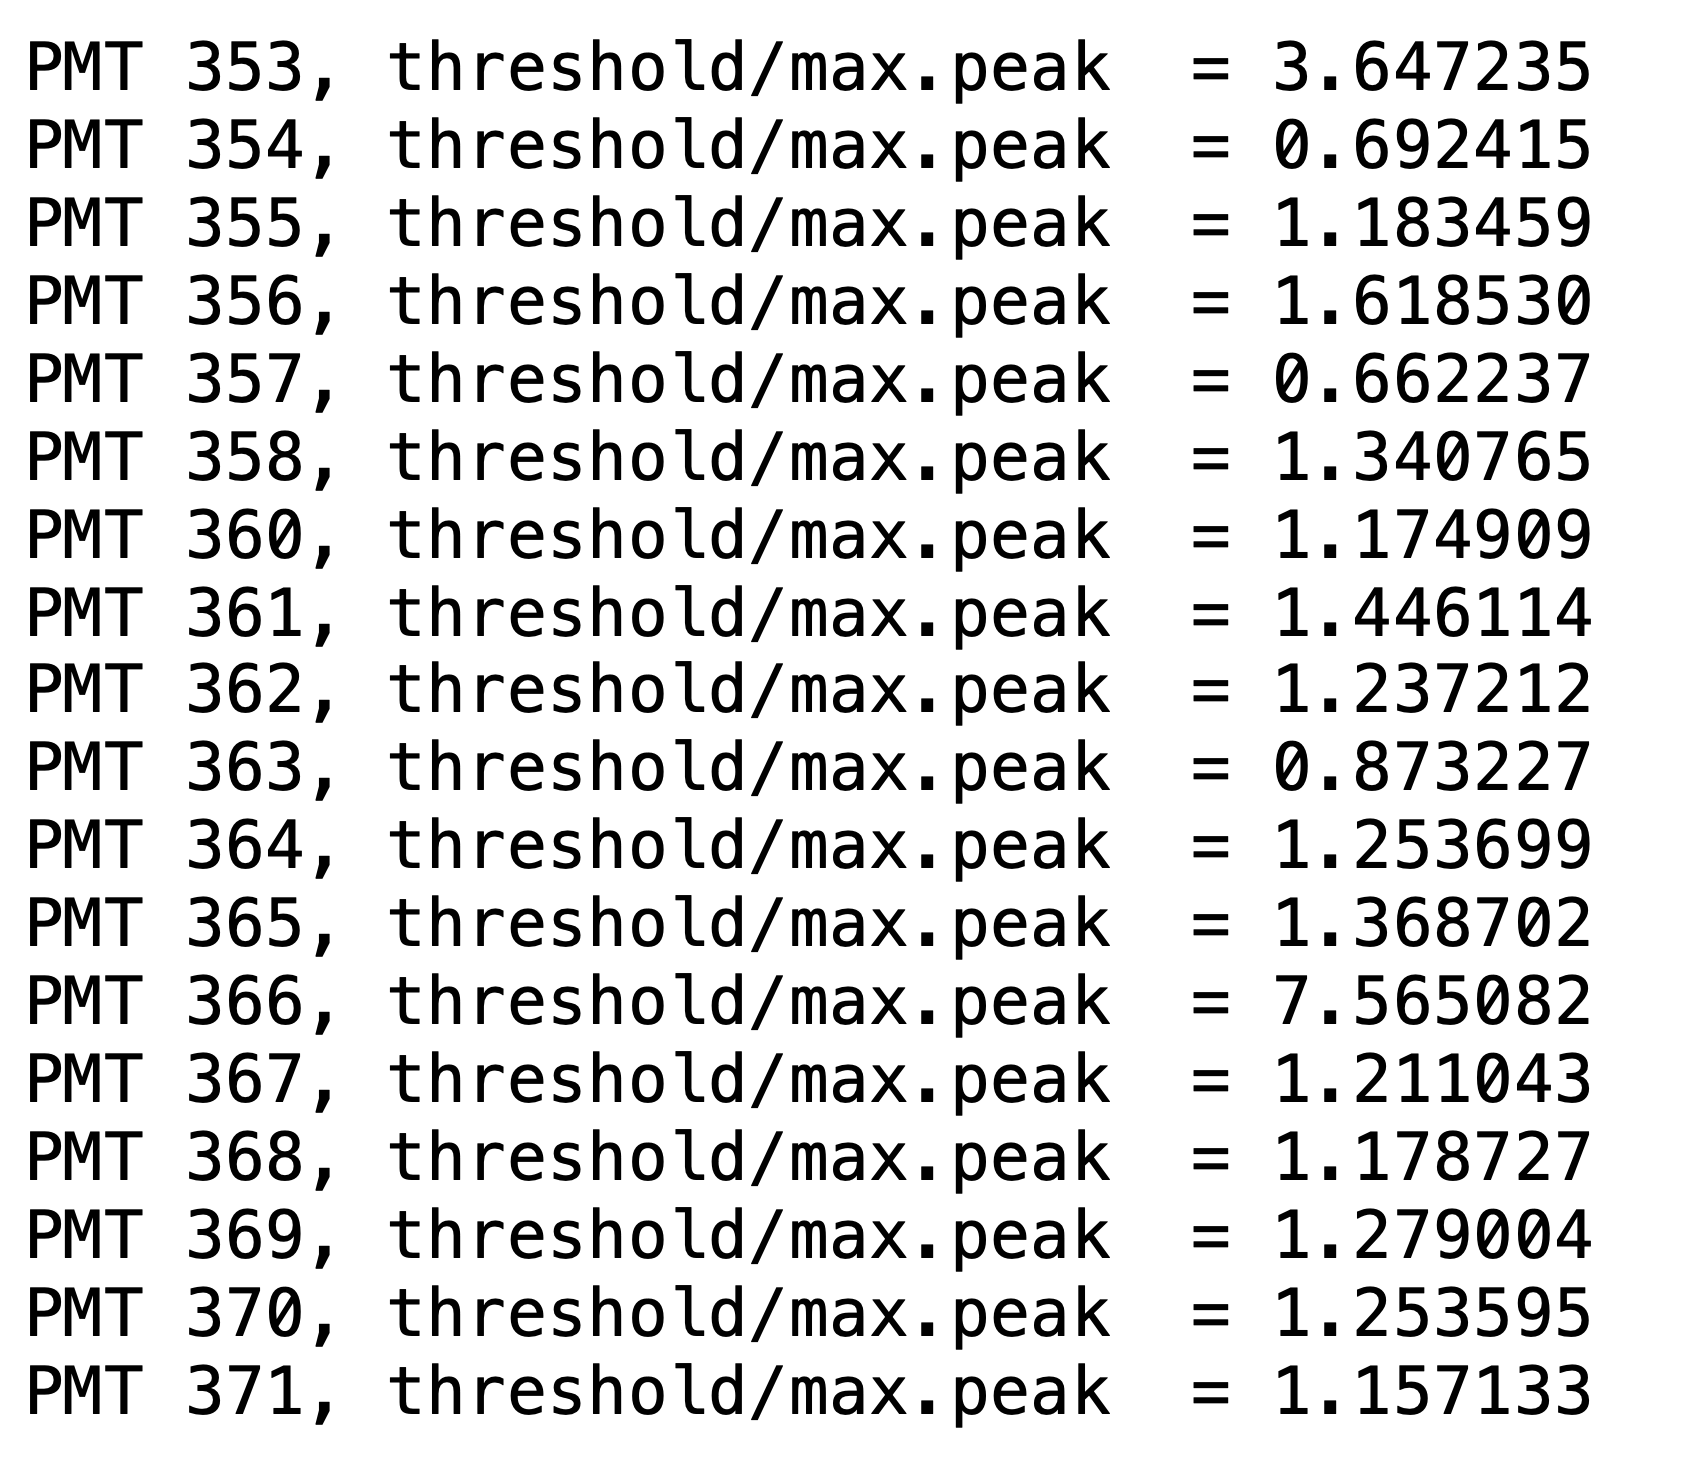
\includegraphics[width=0.8\textwidth, height=4 cm]{ETEL_gain_ratios.png}
	%\caption*{LED}
	\end{subfigure}
\end{figure}
\end{frame}
}


%====================================================
\iffalse
\foreach \n in {Enu,Emu,Pmu,Pmu_z,Pmu_t,ThetaMu,Q2,Ehad,x,y}{
\begin{frame}
	\frametitle{$\n$ Input Histrograms}
\vspace{0.25in}	
\begin{figure}

	\begin{subfigure}{.5\textwidth}
		%\caption*{\scriptsize{Categorized by Truth kinematics}}
	\includegraphics[width=1\textwidth, height=4 cm]{/home/gian/PlotUtils/macros/mnvgeniev1/newbins_mnvgeniev1_\n_Input_InputSmearedData.png}
	\end{subfigure}%
	\begin{subfigure}{.5\textwidth}
	\includegraphics[width=1\textwidth, height=4 cm]{/home/gian/PlotUtils/macros/mnvgeniev1/newbins_mnvgeniev1_\n_Input_TrueData.png}
	\end{subfigure}
\end{figure}
\begin{figure}

	\begin{subfigure}{.5\textwidth}
		%\caption*{\scriptsize{Categorized by Truth kinematics}}
	\includegraphics[width=1\textwidth, height=4 cm]{/home/gian/PlotUtils/macros/mnvgeniev1/newbins_mnvgeniev1_\n_Input_RecoMC.png}
	\end{subfigure}%
	\begin{subfigure}{.5\textwidth}
	\includegraphics[width=1\textwidth, height=4 cm]{/home/gian/PlotUtils/macros/mnvgeniev1/newbins_mnvgeniev1_\n_Input_TruthMC.png}
	\end{subfigure}
\end{figure}
\end{frame}
%====================================================
\begin{frame}
	\frametitle{ $\n$ Matrix and $\chi^{2}$}
\vspace{0.25in}	
\begin{figure}

	%\begin{subfigure}{.5\textwidth}
		%\caption*{\scriptsize{Categorized by Truth kinematics}}
	%\includegraphics[width=1\textwidth, height=4 cm]{/home/gian/PlotUtils/macros/mnvgeniev1/newbins_mnvgeniev1_\n_Input_InputSmearedData.png}
	%\end{subfigure}%
	\begin{subfigure}{.5\textwidth}
	\includegraphics[width=1\textwidth, height=4 cm]{/home/gian/PlotUtils/macros/mnvgeniev1/newbins_mnvgeniev1_\n_Migration_MigrationMatrix.png}
	\end{subfigure}
\end{figure}
\begin{figure}

	\begin{subfigure}{.5\textwidth}
		%\caption*{\scriptsize{Categorized by Truth kinematics}}
	\includegraphics[width=1\textwidth, height=4 cm]{/home/gian/PlotUtils/macros/mnvgeniev1/newbins_mnvgeniev1_\n_Chi2Ratio_2D.png}
	\end{subfigure}%
	\begin{subfigure}{.5\textwidth}
	\includegraphics[width=1\textwidth, height=4 cm]{/home/gian/PlotUtils/macros/mnvgeniev1/newbins_mnvgeniev1_\n_Chi2Ratio_Avg.png}
	\end{subfigure}
\end{figure}
\end{frame}
%====================================================
\begin{frame}
	\frametitle{ $\n$ Matrix and $\chi^{2}$ - logarithmic scale}
\vspace{0.25in}	
\begin{figure}

	%\begin{subfigure}{.5\textwidth}
		%\caption*{\scriptsize{Categorized by Truth kinematics}}
	%\includegraphics[width=1\textwidth, height=4 cm]{/home/gian/PlotUtils/macros/mnvgeniev1_logplots/newbins_mnvgeniev1_\n_Input_InputSmearedData.png}
	%\end{subfigure}%
	\begin{subfigure}{.5\textwidth}
	\includegraphics[width=1\textwidth, height=4 cm]{/home/gian/PlotUtils/macros/mnvgeniev1_logplots/newbins_mnvgeniev1_\n_Migration_MigrationMatrix.png}
	\end{subfigure}
\end{figure}
\begin{figure}

	\begin{subfigure}{.5\textwidth}
		%\caption*{\scriptsize{Categorized by Truth kinematics}}
	\includegraphics[width=1\textwidth, height=4 cm]{/home/gian/PlotUtils/macros/mnvgeniev1_logplots/newbins_mnvgeniev1_\n_Chi2Ratio_2D.png}
	\end{subfigure}%
	\begin{subfigure}{.5\textwidth}
	\includegraphics[width=1\textwidth, height=4 cm]{/home/gian/PlotUtils/macros/mnvgeniev1_logplots/newbins_mnvgeniev1_\n_Chi2Ratio_Avg.png}
	\end{subfigure}
\end{figure}
\end{frame}
}
%====================================================

%====================================================
%====================================================

%====================================================
%====================================================
%=========================================
%====================================================
%=========================================
%==========================================
%=========================================
%===============================================
%===============================================
%===============================================
%===============================================
%===============================================
\fi
\end{document}

%===========================================
%===========================================
%===========================================
%===========================================
%===========================================
%===========================================
%===========================================
%===========================================
%===========================================
%===========================================
%===============================================














































\iffalse
%==============================================
\foreach \n in {12,35,50}{
\begin{frame}
\frametitle{ d\textsuperscript{2}$\sigma$/dxdy}

\centering
%  \scriptsize{Isoscalar correction}\\ 
  \scriptsize{ W$>$2 and Q\textsuperscript{2}$>$1   } \\  
%  \scriptsize{W$>$2}\\

\begin{figure}

  
\begin{subfigure}{.5\textwidth}
  
  \vspace{0.25in}


  \includegraphics[width=1\textwidth, height=3.5cm]{/home/gian/Desktop/Presentations/together/Sept26_Inclusive/plots/Enu_\n_nCTEQ15_Fe_dsigma_dxdy.png}
  
 \caption{nCTEQ15}
\end{subfigure}%
\begin{subfigure}{.5\textwidth}
\vspace{0.25in}


  \includegraphics[width=1\textwidth, height=3.5cm]{/home/gian/Desktop/Presentations/together/Sept26_Inclusive/plots/Enu_\n_GENIE_Fe_dsigma_dxdy.png}
 \caption{GENIE}
\end{subfigure}


\end{figure}


\end{frame}

}
%==========================================================

\foreach \n in {12,35,50}{
\begin{frame}
\frametitle{Normalized  d\textsuperscript{2}$\sigma$/dxdy }

\centering
%  \scriptsize{Isoscalar correction}\\ 
  \scriptsize{ W$>$2 and Q\textsuperscript{2}$>$1   } \\  
%  \scriptsize{W$>$2}\\

\begin{figure}

  
\begin{subfigure}{.5\textwidth}
  
  \vspace{0.25in}


  \includegraphics[width=1\textwidth, height=3.5cm]{/home/gian/Desktop/Presentations/together/Sept26_Inclusive/plots/Enu_\n_nCTEQ15_Fe_dsigma_dxdy_f.png}
  
 \caption{nCTEQ15}
\end{subfigure}%
\begin{subfigure}{.5\textwidth}
\vspace{0.25in}


  \includegraphics[width=1\textwidth, height=3.5cm]{/home/gian/Desktop/Presentations/together/Sept26_Inclusive/plots/Enu_\n_GENIE_Fe_dsigma_dxdy_f.png}
 \caption{GENIE}
\end{subfigure}


\end{figure}


\end{frame}

}

%==================================
\foreach \n in {12,35,50}{
\begin{frame}
\frametitle{ Normalized d$\sigma$/dx}

\centering
%  \scriptsize{Isoscalar correction}\\ 
  \scriptsize{ W$>$2 and Q\textsuperscript{2}$>$1   } \\  
%  \scriptsize{W$>$2}\\

\begin{figure}

  
\begin{subfigure}{.5\textwidth}
  
  \vspace{0.25in}


  \includegraphics[width=1\textwidth, height=3.5cm]{/home/gian/Desktop/Presentations/together/Sept26_Inclusive/plots/Enu_\n_nCTEQ15_Fe_dsigma_dx_f.png}
  
 \caption{nCTEQ15}
\end{subfigure}%
\begin{subfigure}{.5\textwidth}
\vspace{0.25in}


  \includegraphics[width=1\textwidth, height=3.5cm]{/home/gian/Desktop/Presentations/together/Sept26_Inclusive/plots/Enu_\n_GENIE_Fe_dsigma_dx_f.png}
 \caption{GENIE}
\end{subfigure}


\end{figure}


\end{frame}

}

%==================================
\foreach \n in {12,35,50}{
\begin{frame}
\frametitle{Normalized d$\sigma$/dy}

\centering
%  \scriptsize{Isoscalar correction}\\ 
  \scriptsize{ W$>$2 and Q\textsuperscript{2}$>$1   } \\  
%  \scriptsize{W$>$2}\\

\begin{figure}

  
\begin{subfigure}{.5\textwidth}
  
  \vspace{0.25in}


  \includegraphics[width=1\textwidth, height=3.5cm]{/home/gian/Desktop/Presentations/together/Sept26_Inclusive/plots/Enu_\n_nCTEQ15_Fe_dsigma_dy_f.png}
  
 \caption{nCTEQ15}
\end{subfigure}%
\begin{subfigure}{.5\textwidth}
\vspace{0.25in}


  \includegraphics[width=1\textwidth, height=3.5cm]{/home/gian/Desktop/Presentations/together/Sept26_Inclusive/plots/Enu_\n_GENIE_Fe_dsigma_dy_f.png}
 \caption{GENIE}
\end{subfigure}


\end{figure}


\end{frame}

}

%==================================
%=====================================
\foreach \n in {12,35,50}{

\begin{frame}
\frametitle{  d\textsuperscript{2}$\sigma$/dxdy ratios for nCTEQ15/GENIE $<$ 3}

\centering
%  \scriptsize{Isoscalar correction}\\ 
  \scriptsize{ W$>$2 and Q\textsuperscript{2}$>$1   } \\  
%  \scriptsize{W$>$2}\\

\begin{figure}
  
  \vspace{0.25in}
  \includegraphics[width=0.8\textwidth, height=5 cm]{/home/gian/Desktop/Presentations/together/Sept26_Inclusive/plots/ratio_Enu_\n_nCTEQ15_Fe_Enu_\n_genie_Fe_dsigma_dxdy_overflow.png}
  
\end{figure}

\end{frame}

}
%=========================================

%=====================================
\foreach \n in {12,35,50}{

\begin{frame}
\frametitle{  d$\sigma$/dx ratios for nCTEQ15/GENIE  }

\centering
%  \scriptsize{Isoscalar correction}\\ 
  \scriptsize{ W$>$2 and Q\textsuperscript{2}$>$1   } \\  
%  \scriptsize{W$>$2}\\

\begin{figure}
  
  \vspace{0.25in}
  \includegraphics[width=0.8\textwidth, height=5 cm]{/home/gian/Desktop/Presentations/together/Sept26_Inclusive/plots/ratio_Enu_\n_nCTEQ15_Fe_Enu_\n_genie_Fe_dsigma_dx.png}
  
\end{figure}

\end{frame}

}
%=========================================
%=====================================
\foreach \n in {12,35,50}{

\begin{frame}
\frametitle{  d$\sigma$/dy ratios for nCTEQ15/GENIE}

\centering
%  \scriptsize{Isoscalar correction}\\ 
  \scriptsize{ W$>$2 and Q\textsuperscript{2}$>$1   } \\  
%  \scriptsize{W$>$2}\\

\begin{figure}
  
  \vspace{0.25in}
  \includegraphics[width=0.8\textwidth, height=5 cm]{/home/gian/Desktop/Presentations/together/Sept26_Inclusive/plots/ratio_Enu_\n_nCTEQ15_Fe_Enu_\n_genie_Fe_dsigma_dy.png}
  
\end{figure}

\end{frame}

}
%=========================================
%=====================================
\foreach \n in {12,35,50}{

\begin{frame}
\frametitle{  d$\sigma$/dy ratios for nCTEQ15/GENIE (zoom)}

\centering
%  \scriptsize{Isoscalar correction}\\ 
  \scriptsize{ W$>$2 and Q\textsuperscript{2}$>$1   } \\  
%  \scriptsize{W$>$2}\\

\begin{figure}
  
  \vspace{0.25in}
  \includegraphics[width=0.8\textwidth, height=5 cm]{/home/gian/Desktop/Presentations/together/Sept26_Inclusive/plots/ratio_Enu_\n_nCTEQ15_Fe_Enu_\n_genie_Fe_dsigma_dy_zoom.png}
  
\end{figure}

\end{frame}

}
%=========================================

%=====================================

\fi











